\documentclass[a4paper,11pt]{article}
\usepackage[utf8]{inputenc}
\usepackage{tikz}
\usepackage{amsmath} \usepackage{amssymb}
\usepackage{amsfonts}
%\usepackage{amscd}
\usepackage{latexsym} \usepackage{mathrsfs} 

\usepackage{ngerman}
\usepackage{yfonts}
\usepackage{color}
%\usepackage[pdftex]{graphicx}
%\usepackage{pdfpages}
\usepackage{dsfont}
\usepackage{xy}\xyoption{all}
\usepackage{enumitem}


%%%%%%%%
\usepackage{graphicx}
\definecolor{MNTFcol}{RGB}{0,101,97}
\definecolor{dunkelgrau}{rgb}{0.5,0.5,0.5}
\definecolor{hellgrau}{rgb}{0.95,0.95,0.95}
\definecolor{neuePO}{rgb}{0.85,0.85,0.94}
\definecolor{purp4}{rgb}{0.36,0.28,0.55}
\definecolor{silv}{rgb}{0.45,0.45,0.50}
\usepackage{colortbl}


\setlength{\textwidth}{18cm} %% eigentlich 16cm
\setlength{\oddsidemargin}{-10mm} %%eigentlich 0mm
\setlength{\evensidemargin}{0mm}
\setlength{\unitlength}{1mm}
\setlength{\textheight}{22cm}
%\voffset=-3cm

\renewcommand{\familydefault}{\sfdefault}
\usepackage{helvet}

\def\R{{\mathbb R}} \def\C{{\mathbb C}} \def\N{{\mathbb N}}
\def\Z{{\mathbb Z}} \def\Pj{{\mathbb P}} \def\cc{{\cal C}}
\def\Q{{\mathbb Q}} \def\vi{\varphi} \def\ve{\varepsilon}
\def\F{{\mathbb F}}
\newcommand{\cO}{\mathcal{O}}
\newcommand{\cM}{\mathcal{M}}
\newcommand{\cN}{\mathcal{N}}
\newcommand{\cF}{\mathcal{F}}
\newcommand{\cG}{\mathcal{G}}
\newcommand{\cH}{\mathcal{H}}
\newcommand{\cHom}{\mathcal{H}om}
\newcommand{\GL}{\mathrm{GL}}
\newcommand{\Ab}{\mathcal{A}b}

\newcommand{\falle}[1]{\underset{{#1}}{\forall} \ }
\newcommand{\gibts}[1]{\underset{{#1}}{\exists} \ }


\newcommand{\lto}{\longrightarrow}
\newcommand{\widebar}[1]{\overline{#1}}
\newcounter{aufg}
\newcommand{\Aufg}{\stepcounter{aufg}\vspace*{0.2cm}\noindent{\bf
    Aufgabe \arabic{aufg}:} }
\newcommand{\tAufg}{\stepcounter{aufg}\vspace*{0.2cm}\noindent{\bf
    "U.Aufgabe \arabic{aufg}:} }

\newcommand{\sAufg}{\vspace*{0.7cm}\noindent{\bf $\ast $-Aufgabe:} }
\renewcommand{\labelenumi}{{\rm \roman{enumi})}}

\newcommand{\sRHom}{\mathrm{R}\mathcal{H}om}
\newcommand{\Hom}{\text{Hom}}
\newcommand{\cB}{\mathcal{B}}
\newcommand{\cA}{\mathcal{A}}
\newcommand{\cD}{\mathcal{D}}
\newcommand{\cC}{\mathcal{C}}
\newcommand{\cL}{\mathcal{L}}
\newcommand{\eig}[1]{\mathrm{Eigenwerte}(#1)}
\newcommand{\isoto}{\stackrel{\cong}{\lto}}
\newcommand{\companion}[1]{\mathrm{Begleit}(#1)}
\newcommand{\sbt}{\text{\tiny$\bullet$}}
\newcommand{\Kom}{\mathrm{Kom}}

\begin{document}
\sffamily
\setlist[enumerate]{leftmargin=*}

\pagestyle{empty}

\unitlength1mm

\begin{picture}(100,50)

\put(-8,52){
\includegraphics[scale=0.4]{Uni_Aug_Logo_MNTF_RGB}}

\put(110,82){
\begin{minipage}[t]{6cm} \baselineskip10pt
 \rule[2.5mm]{6cm}{.3pt}
 
  {\scriptsize\bf  Prof. Dr. Marco Hien\\
  M. Sc. Thomas Bargen\\
 \rule{6cm}{.3pt}}
\end{minipage}
}
\end{picture}

\vspace*{-6.5cm}
\centerline{\Large Aufgaben zu {\it Riemannsche Flächen} -- WS 2025/26}


\medskip \centerline{10. Blatt}


\setcounter{aufg}{30}
\newcounter{labl}

\vspace*{1cm}

\Aufg Sei $\mathscr{U}$ eine offene Überdeckung von $X$ und $\mathcal{F}$ eine Garbe abelscher Gruppen auf $X$. Zeigen Sie exemplarisch, dass
\[
\delta\circ\delta:\check{C}^0(\mathscr{U},\mathcal{F})\longrightarrow\check{C}^1(\mathscr{U},\mathcal{F})\longrightarrow\check{C}^2(\mathscr{U},\mathcal{F})
\]
der Null-Morphismus ist.

\vspace{0.5em}

\Aufg Seien $\mathscr{W}\le\mathscr{V}\le\mathscr{U}$ jeweils Verfeinerungen offener Überdeckungen. Zeigen Sie, dass die Verfeinerungsabbildungen in Čech-Kohomologie wie erwartet kommutieren, das heißt, dass das folgende Dreieck kommutiert:
\begin{center}
	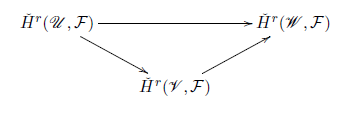
\includegraphics[scale=0.8]{diag}
\end{center}

\Aufg Zeigen Sie, dass die Verfeinerungsabbildung auf Čech-Kohomologie
\[
\check{H}^r(\mathscr{U},\mathcal{F}) \longrightarrow \check{H}^r(\mathscr{V},\mathcal{F})
\]
für eine Verfeinerung $\mathscr{V}\le\mathscr{U}$ immer injektiv ist.

\vspace{0.5em}

\Aufg Betrachten Sie die Garben $\mathcal{O}(m)$ auf $\mathbb{CP}^1$ aus Aufgabe 10, Blatt 3. Sei $\mathscr{U}=(U_0,U_1)$ die dort betrachtete offene Überdeckung (die Standard-Kartengebiete auf $\mathbb{CP}^1$). Zeigen Sie, dass\footnote{Beachten Sie, dass diese Kohomologiegruppen in natürlicher Weise $\mathbb{C}$-Vektorräume sind, weil die lokalen Schnitte $\mathcal{O}(m)(U)$ dies sind und die Korand-Operatoren $\delta$ offenbar $\mathbb{C}$-linear.}
\[
\dim_{\mathbb{C}} \check{H}^1(\mathscr{U},\mathcal{O}(m)) \;=\;
\begin{cases}
	-m-1 & \text{für } m\le -2,\\[4pt]
	0 & \text{für } m\ge -1.
\end{cases}
\]



\end{document}
